\documentclass{article}
\usepackage[utf8]{inputenc}
\usepackage[letterpaper, portrait, margin=1in]{geometry}
\usepackage{enumerate}
% Display only levels as deep as subsection in tableofcontents
\setcounter{tocdepth}{2}

\usepackage{caption}
\usepackage{graphicx}
\graphicspath{ {images/} }
\usepackage{array}

\usepackage{multirow,booktabs}

% Define function subcommands
\newcommand{\name}[1]{\hline \multicolumn{2}{|l|}{\texttt{#1}} }
\newcommand{\inp}[1]{\hline \textbf{Input:} & #1}
\newcommand{\out}[1]{\hline \textbf{Output:} & #1}
\newcommand{\desc}[1]{\hline \textbf{Description:} & #1 }

% Define function command
\newcommand{\fcn}[4]{
    \begin{center}
    \begin{tabular}{|p{2cm} p{10cm}|}
    \hline
    \name{#1} \\
    \inp{#2} \\
    \out{#3} \\
    \desc{#4} \\
    \hline
    \end{tabular}
    \end{center}
}

%%%%%%%%%%%%%%%%%%%%%%%%%%%%%%%%%%%%%%%%%%%%%%%%%%%%%%%%%%%%%%%%%%%%%%%%%%%%%
% GRAPHS
%%%%%%%%%%%%%%%%%%%%%%%%%%%%%%%%%%%%%%%%%%%%%%%%%%%%%%%%%%%%%%%%%%%%%%%%%%%%%
\usepackage{tikz}
\usepackage{verbatim}
\usetikzlibrary{positioning,arrows,shapes}
%%%%%%%%%%%%%%%%%%%%%%%%%%%%%%%%%%%%%%%%%%%%%%%%%%%
% HEADER
%%%%%%%%%%%%%%%%%%%%%%%%%%%%%%%%%%%%%%%%%%%%%%%%%%%
\usepackage{fancyhdr}
\pagestyle{fancy}
\fancyhf{}
\fancyhead[C]{PiSonal Trainer: Weight Lifting Performance Tracker}
\fancyfoot[L]{System Architecture}
\fancyfoot[R]{\thepage}
\renewcommand{\headrulewidth}{0.4pt}
\renewcommand{\footrulewidth}{0.4pt}

% Use this to pad tables
\usepackage{array}
\setlength\extrarowheight{6pt}

% Define tab command
\newcommand\tab{\hspace*{2cm}}


%%%%%%%%%%%%%%%%%%%%%%%%%%%%%%%%%%%%%%%%%%%%%%%%%%%
% TITLE
%%%%%%%%%%%%%%%%%%%%%%%%%%%%%%%%%%%%%%%%%%%%%%%%%%%
\title{
PiSonal Trainer: Weight Lifting Performance Tracker\\
\Large {System Architecture}
}
\date{January 11, 2017}
\author{Birunthaa Umamahesan \and Micaela Estabillo \and Simarpreet Singh}

\begin{document}
%%%%%%%%%%%%%%%%%%%%%%%%%%%%%%%%%%%%%%%%%%%%%%%%%%%
% COVER PAGE
%%%%%%%%%%%%%%%%%%%%%%%%%%%%%%%%%%%%%%%%%%%%%%%%%%%
\thispagestyle{plain}
\pagenumbering{gobble}
\maketitle
\vfill
\begin{center}
    Prepared for Computer Science 4ZP6: Capstone Project \\
    Instructor: Dr. Wenbo He
    Fall/Winter 2016-2017\\
\end{center}
\newpage

%%%%%%%%%%%%%%%%%%%%%%%%%%%%%%%%%%%%%%%%%%%%%%%%%%%
% TABLE OF CONTENTS AND REVISION HISTORY
%%%%%%%%%%%%%%%%%%%%%%%%%%%%%%%%%%%%%%%%%%%%%%%%%%%
\tableofcontents

\listoffigures

\listoftables

\thispagestyle{plain}
\pagenumbering{gobble}

\newpage

\section*{Revision History}
\begingroup
\begin{tabular}{ | p{2cm} | p{1.5cm} | p{3.8cm} | p{7cm} |} 
    \hline
    \textbf{Date} & \textbf{Version} & \textbf{Primary Author} & \textbf{Comment}\\
    \hline
    1/11/2017 & 1.00 & Birunthaa Umamahesan & Proofread document for revision 0\\
    \hline
    1/11/2017 & 1.00 & Micaela Estabillo & Finalize document draft\\
    \hline
    1/9/2017 & 1.00 & Micaela Estabillo & Create document outline\\
    \hline
\end{tabular}
    \captionof{table}{Revision history}
\endgroup


\begin{center}
% Volere Edition 16
%We acknowledge that this document uses material from the Volere Requirements Specification Template, copyright © 1995 – 2012 the Atlantic Systems Guild Limited.
\end{center}

\newpage

\clearpage
\setcounter{page}{1}
\pagenumbering{arabic}

%%%%%%%%%%%%%%%%%%%%%%%%%%%%%%%%%%%%%%%%%%%%%%%%%%%
% 
%%%%%%%%%%%%%%%%%%%%%%%%%%%%%%%%%%%%%%%%%%%%%%%%%%%

\section{Introduction and Overview}
This document provides a description of how PiSonal Trainer will be built. The following are covered in this document:
\begin{itemize}
    %\item An explanation of the templates, symbols and conventions used in the document
    \item Diagram and individual descriptions of the overall component decomposition of the system
    \item Anticipated and unlikely design changes
    \item The Requirements and Design Traceability Matrix relating the system’s components to the project requirements established in the Software Requirements Specifications (SRS) document
\end{itemize}

\section{Templates, Symbols and Conventions Used}
The modules' functions are specified in the format shown in Table 2. This is used in the Detailed Design document.

\begingroup
\begin{center}
\fcn
{nameOfFunction()}
{List of input variables or actions}
{List of updated variables or system's response}
{Description of what the function does}
\end{center}
\captionof{table}{Function specification format}
\endgroup


\section{Decomposition into Components}
The system is decomposed based on its different elements in order to allow each component to be implemented and developed independently. Nevertheless, each component interacts with at least one other.
\begin{enumerate}
\item \textbf{User Interface (UI)}: The UI encompasses the frontend and backend of the mobile app used to track workouts and display performance history. The app communicates with the database containing a collection of authorized users to authenticate. It also sends exercise performance statistics to the database. A mobile platform is ideal for PiSonal Trainer so that users can easily bring their device to their gyms, and record or view their performance.

\item \textbf{Camera and Counting Algorithm}: Since the camera in use is a Macbook webcam, the movement counting algorithm is implemented on the same machine using OpenCV-python. This is done to reduce resource overhead that would be generated by sending image information for processing to a remote server. The algorithm is discussed in detail in the Detailed Design document.

\item \textbf{Database}: The database keeps unauthorized users from using the app and stores counts pertaining to a user's exercises. User performance graphs are dynamically generated by querying the database and sending data back to the user's phone. All the counts are stored in the database in order to avoid taking up too much space in the phone's disk.
\end{enumerate}

\newpage

\begingroup
\begin{center}
\begin{figure}[h]
\center{
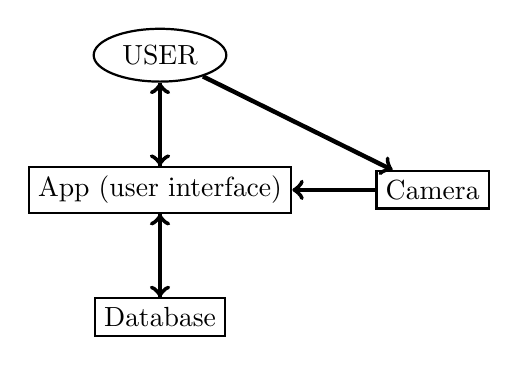
\begin{tikzpicture} [node distance=30pt]
    \node[draw,thick,ellipse] (user) {USER};
    \node[draw,thick,rectangle,below=of user] (ui) {App (user interface)};
    \node[draw,thick,rectangle,below=of ui] (db) {Database};
    \node[draw,thick,rectangle,right=of ui] (camera) {Camera};

    \path (user) edge [->,ultra thick] (ui);
    \path (ui) edge [->,ultra thick] (user);
    \path (ui) edge [->,ultra thick] (db);
    \path (db) edge [->,ultra thick] (ui);
    \path (user) edge [->,ultra thick] (camera);
    \path (camera) edge [->,ultra thick] (ui);
\end{tikzpicture}
}\end{figure}
\end{center}
\captionof{figure}{Interaction of PiSonal Trainer Components}
\endgroup

\section{Anticipated Changes}
%(Anticipated changes and Components Traceability needed)
The expected changes will be caused by changing the system camera from a Macbook webcam to the mobile phone's built-in camera. The new interaction diagram of the components is illustrated in Figure 2.
\begin{enumerate}
    \item \textbf{Use phone's built-in camera}: Merge the camera component into the mobile app so vision and movement detection can be performed within the app instead of an external webcam and computer. To track movement using the user's phone, the counting algorithm would have to be ported to JavaScript as well.
    \item \textbf{Add a camera tab to existing mobile app}: The app currently only allows manually typing in the number of reps/sets for an exercise and a weight. This feature will be retained, but a new tab for recording performance metrics using the phone camera will be added. Using the camera for inputting counts assumes that the gym equipment will be colour-coded according to weight, thereby removing the need for manual input.
\end{enumerate}


\begingroup
\begin{center}
\begin{figure}[h]
\center{
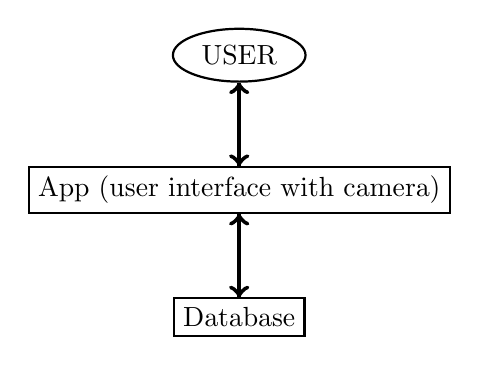
\begin{tikzpicture} [node distance=30pt]
    \node[draw,thick,ellipse] (user) {USER};
    \node[draw,thick,rectangle,below=of user] (ui) {App (user interface with camera)};
    \node[draw,thick,rectangle,below=of ui] (db) {Database};

    \path (user) edge [->,ultra thick] (ui);
    \path (ui) edge [->,ultra thick] (user);
    \path (ui) edge [->,ultra thick] (db);
    \path (db) edge [->,ultra thick] (ui);
\end{tikzpicture}
}
\end{figure}
\end{center}
\captionof{figure}{Interaction of PiSonal Trainer Components After Changing Camera}
\endgroup

\section{Unlikely Changes}
\begin{enumerate}
    \item \textbf{User interface layout}: The general look of the mobile app is unlikely to change, even after adding the camera tab (see Anticipated Change 1).
    \item \textbf{Movement detection algorithm}: The algorithm behind the rep/set counting mechanism of the system will likely stay the same even after porting the Python code to JavaScript in order to use a mobile camera.
\end{enumerate}

\newpage
\section{Requirements and Design Traceability Matrix}
The following table contains the functional requirements identified in PiSonal Trainer's Software Requirement Specification document, their descriptions and their corresponding design component/s.
\begingroup
\begin{center}
\begin{tabular}{| p{2.5cm} | p{7cm} | p{3.5cm} |}
    \hline
    \textbf{Requirement} & \textbf{Description} & \textbf{Design Reference} \\
    \hline
    R1 & A QR code attached to gym equipment shall be scanned using the app & UI \\
    R2 & The app shall be able to identify the equipment’s weight & UI \\
    R3 & Only registered users may be able to use the app & UI, Database\\
    R4 & The app shall provide meaningful error messages & UI \\
    R5 & The app shall display the user’s progress statistics through visual graphs & UI, Database \\
    R6 & A camera shall track the motion of the gym equipment & Camera\\
    R7 & The user’s exercise performance data shall be stored for future retrieval & Database \\
    R8 & The user’s performance shall be calculated using data from the camera and the equipment’s weight & UI, Database, Camera \\
    \hline
\end{tabular}
\end{center}
\captionof{table}{Requirements and Design Traceability}
\endgroup


%%%%%%%%%%%%%%%%%%%%%%%%%%%%%%%%%%%%%%%%%%%%%%%%%%%
% REFERENCES
%%%%%%%%%%%%%%%%%%%%%%%%%%%%%%%%%%%%%%%%%%%%%%%%%%%
% \section*{References}

%%%%%%%%%%%%%%%%%%%%%%%%%%%%%%%%%%%%%%%%%%%%%%%%%%%
% INDEX
%%%%%%%%%%%%%%%%%%%%%%%%%%%%%%%%%%%%%%%%%%%%%%%%%%%
%\section*{Index}

\end{document}

The document should include the system architecture design and component design. You should give the architecture of the system, system components, APIs, algorithms used, solutions to address the challenges mentioned in your previous report, and shows the reasons on your design choices.
